\appendix

\section{System Prompts for Two-Pass Evaluation}
\label{app:system_prompts}

To enable accurate reproduction of our results and clarify the evaluation setup described in \S\ref{sec:two_pass_estimation}, we provide the complete system prompts used in our experiments. We use consistent formatting instructions across all prompts to standardize outputs, and we include in-context learning examples to ensure stable model behavior and syntactically correct answers in the required format.

\paragraph{Second Pass System Prompt.}
As described in \S\ref{sec:two_pass_estimation}, the second pass forces models to answer questions that were refused in the first pass. We combine explicit instructions with in-context examples to enforce the output format and minimize formatting errors. Since most models we evaluate rarely refuse when given such instructions, we simply tell the model to always provide an answer. The in-context examples below help the model consistently produce the required XML-style tags. We show the complete second-pass system prompt used in our experiments:

\begin{lstlisting}
Second Pass Prompt

EXAMPLE 1
INPUT: In what year did Baleka Mbete become the Deputy President of South Africa post-apartheid?
OUTPUT: <answer>2008</answer>

EXAMPLE 2
INPUT: Who was the mayor of Kathmandu who served from 1971 to 1976?
OUTPUT: <answer>Rajendra Man Suwal</answer>

[omitted for brevity]

EXAMPLE 10
INPUT: The book "Rhine" by Anselm Kiefer is from what year?
OUTPUT: <answer>1981</answer>

Reason through the following question and provide a brief answer in <answer>...</answer> at the end. You always give an answer and you never return <answer>UNANSWERED</answer>.

Question: {question}
\end{lstlisting}

\paragraph{First Pass System Prompt.}
Our first-pass prompts use the same design and formatting as the second-pass prompt but make small, targeted changes to the instruction wording and the mix of in-context examples to encourage appropriate refusal behavior (see \S\ref{sec:refusal_index_method} and \S\ref{sec:two_pass_estimation}). We show one complete first-pass prompt variant below; other variants differ only in how strongly they encourage refusal and the proportion of examples that show returning \verb|<answer>UNANSWERED</answer>| when uncertain. Due to space constraints, we do not include the remaining variants in full.

\begin{lstlisting}
First Pass Prompt -- Highest Refusal Tendency

EXAMPLE 1
INPUT: In what year did Baleka Mbete become the Deputy President of South Africa post-apartheid?
OUTPUT: <answer>UNANSWERED</answer>

[omitted for brevity]

EXAMPLE 10
INPUT: The book "Rhine" by Anselm Kiefer is from what year?
OUTPUT: <answer>UNANSWERED</answer>

Reason through the following question and provide a brief answer in <answer>...</answer> at the end. You are very cautious and need good evidence before drawing conclusions. You prefer saying you don't know by returning <answer>UNANSWERED</answer> rather than risking a wrong answer.

Question: {question}
\end{lstlisting}

As described in \S\ref{sec:validating_latent_uncertainty_model}, these first-pass variants differ from the second pass in only two ways: (1) how strongly the instruction encourages refusal and (2) the proportion of \verb|<answer>UNANSWERED</answer>| responses in the in-context examples. Together, these changes control the overall refusal tendency without otherwise changing the task.

\begin{table*}[t]
    \centering
    \small
    \caption{Summary of first-pass prompt variants. Only the refusal instruction and the proportion of UNANSWERED responses differ across variants; all other elements match the second-pass prompt. Ratios vary by model and dataset (see \S\ref{sec:simpleqa_evaluation}); we report relative levels for brevity.}
    \label{tab:first_pass_prompt_variants}
    \begin{tabularx}{\textwidth}{l X c}
        \toprule
        \textbf{Type} & \textbf{Instruction} & \textbf{UNANSWERED ratio} \\
        \midrule
        Least Refusal & You only give an answer if you are confident; otherwise you return $<$answer$>$UNANSWERED$<$/answer$>$. & 0.00 \\
        Moderate Refusal & You are cautious and may return \texttt{UNANSWERED} when unsure. & 0.10 \\
        High Refusal & You make reasonable guesses from partial information but avoid speculation; return \texttt{UNANSWERED} if not very confident. & 0.40 \\
        Highest Refusal & You are very cautious and prefer \texttt{UNANSWERED} rather than risking a wrong answer. & 0.60 \\
        \bottomrule
    \end{tabularx}
\end{table*}

\section{Validating the Gaussian Copula Assumption}
\label{app:copula_validation}

To model the joint dependence between refusal and incorrectness under forced answering in the main text, we use the bivariate normal copula (Gaussian copula). This choice allows us to estimate the Refusal Index by capturing the correlation structure between the latent refusal score and question difficulty while remaining agnostic to the marginal distributions. However, it is important to validate whether this distributional assumption is appropriate for real model behavior.

In this section, we compare the Gaussian copula against three alternative copula families to determine which provides the best fit for modeling refusal behavior. We consider Student-\emph{t}, Gumbel, and Clayton copulas as alternatives, each capturing different forms of dependence structure. We evaluate which copula family best fits the observed refusal patterns across multiple models and prompts.


\paragraph{Evaluation Criteria.}
We use two criteria to evaluate copula performance: goodness-of-fit and win-rate comparisons between the guassian copula and the alternatives.
Since the margins are fixed by construction in our two-pass evaluation setup, the natural goodness-of-fit criterion is the multinomial log-likelihood implied by each copula through the resulting 2\,$\times$\,2 cell probabilities. However, since different copulas have varying numbers of parameters (e.g., Student-\emph{t} has 2 parameters while Gaussian has only 1), we must penalize model complexity to ensure fair comparison. We complement the raw log-likelihood with the Akaike Information Criterion (AIC) and Bayesian Information Criterion (BIC):
\begin{align}
\text{AIC} &= 2k - 2\ell(\hat{\theta})\\
\text{BIC} &= k\log(n) - 2\ell(\hat{\theta})
\end{align}
where $k$ is the number of parameters, $n$ is the sample size, and $\ell(\hat{\theta})$ is the maximized log-likelihood. These criteria penalize more complex dependence structures, providing a principled basis for model selection\textbf{}.
For the second criterion, we evaluate win rates by comparing how often the Gaussian copula outperforms each alternative across different model-prompt combinations. 
To challenge the Gaussian choice, we compare it with three standard alternatives that capture different forms of dependence. A Student-\emph{t} copula adds a heavy-tail parameter to the Gaussian structure; a Clayton copula emphasizes lower-tail association and is asymmetric; and a Gumbel copula emphasizes upper-tail association and is also asymmetric. All candidates are fit by maximum likelihood with margins fixed at the empirical refusal and forced-answering error rates for each model-prompt combination. Win rates are computed across these individual model-prompt units to assess the relative performance of each copula family.

\paragraph{Experimental Setup.}
We systematically evaluate and compare the maximum log-likelihood for each copula family on the SimpleQA dataset. Our evaluation covers all 17 models and 4 first-pass prompts used in the main evaluation (see \S\ref{sec:simpleqa_evaluation}). 
For each model-prompt combination, we obtain a 2\,$\times$\,2 contingency table with margins $(r,\mu)$ representing the refusal rate and error rate respectively. Each copula $C$ maps these margins to cell probabilities $(p_{00},p_{01},p_{10},p_{11})$, and we estimate the copula parameters by maximizing the multinomial likelihood of the observed counts as defined in Equation~\ref{eq:mle}:
\begin{align}
\hat{\rho} &= \argmax_{\rho \in (-1,1)} \ell(\rho) \nonumber\\
\text{where} \quad \ell(\rho) &= \sum_{a,b\in\{0,1\}} n_{ab} \log p_{ab}(\rho) \label{eq:mle}
\end{align}
This setup isolates the copula choice while maintaining consistency with the main evaluation framework.

\begin{table*}[t]
  \centering
  \small
  \caption{Copula comparison on SimpleQA across model-prompt combinations (ties counted as 0.5). Left panel reports mean goodness-of-fit metrics across all combinations for each copula family. Right panel reports the fraction of combinations where the Gaussian copula outperforms each alternative.}
  \label{tab:copula_comparison}
  \begin{minipage}[t]{0.48\textwidth}
    \centering
    \textbf{Goodness-of-Fit Metrics}
    \begin{tabular}{@{}lccc@{}}
      \toprule
      Family & Log-likelihood & AIC & BIC \\
      \midrule
      Gaussian & $-1832.08$ & $3666.16$ & $3671.76$ \\
      Student-\emph{t} & $-1859.14$ & $3722.27$ & $3733.48$ \\
      Gumbel & $-2086.86$ & $4175.72$ & $4181.32$ \\
      Clayton & $-2200.13$ & $4402.26$ & $4407.86$ \\
      \bottomrule
    \end{tabular}
  \end{minipage}
  \hfill
  \begin{minipage}[t]{0.48\textwidth}
    \centering
    \textbf{Gaussian Win Rates}
    \begin{tabular}{@{}lccc@{}}
      \toprule
      Versus & Log-likelihood & AIC & BIC \\
      \midrule
      Student-\emph{t} & $1.000$ & $1.000$ & $1.000$ \\
      Clayton & $0.676$ & $0.647$ & $0.647$ \\
      Gumbel & $0.632$ & $0.618$ & $0.618$ \\
      \bottomrule
    \end{tabular}
  \end{minipage}
\end{table*}

The results in Table~\ref{tab:copula_comparison} indicate that the Gaussian copula provides the strongest average fit and, after accounting for complexity, the best overall trade-off between parsimony and data fit. The Student-\emph{t} copula, despite its additional heavy-tail parameter, does not improve the average log-likelihood and is uniformly worse once complexity penalties are applied. This aligns with intuition for 2\,$\times$\,2 data with fixed margins, where heavy tails are weakly identified and tend to degenerate toward the Gaussian case. The asymmetric Clayton and Gumbel copulas trail substantially on both raw fit and information criteria, though they can win occasionally on individual units.

\paragraph{Conclusion.} We choose the Gaussian copula for two primary reasons: (1) it provides the better average fit across model-prompt combinations as evidenced by superior log-likelihood, AIC, and BIC scores; and (2) it is the simplest and most interpretable copula family, requiring only a single correlation parameter while making minimal distributional assumptions about the dependence structure.
In summary, the bivariate normal copula is both simple and sufficiently accurate for the refusal--incorrectness dependence considered here. Its combination of low assumptions and competitive fit makes it a natural default for estimating the Refusal Index.

\section{Results on SimpleQA}

\begin{table*}[t]
    \centering
    \tiny
    \caption{Results on SimpleQA with 95\% CI.}
    \label{tab:simpleqa_model_comparison}
    \begin{tabularx}{\textwidth}{X c c c c c c}
    \toprule
    \textbf{Model} & \textbf{Accuracy} & \textbf{Refusal} & \textbf{C / A} & \textbf{F-score} & \textbf{Weighted} & \textbf{Refusal Index} \\
    \midrule
    Qwen2.5-72B                    & 0.05 [0.04, 0.05] & 0.74 [0.73, 0.75] & 0.20 [0.18, 0.22] & 0.07 [0.07, 0.08] & -0.21 [-0.22, -0.20] & 0.49 [0.45, 0.53] \\
    Qwen3-32B                      & 0.03 [0.03, 0.03] & 0.68 [0.67, 0.69] & 0.12 [0.10, 0.15] & 0.05 [0.04, 0.05] & -0.29 [-0.29, -0.28] & 0.34 [0.28, 0.40] \\
    Qwen3-32B-Think                & 0.04 [0.03, 0.04] & 0.71 [0.70, 0.72] & 0.14 [0.13, 0.16] & 0.06 [0.05, 0.06] & -0.25 [-0.26, -0.24] & 0.34 [0.29, 0.39] \\
    Qwen3-235B                     & 0.38 [0.37, 0.39] & 0.36 [0.35, 0.37] & 0.59 [0.58, 0.61] & 0.45 [0.44, 0.46] & -0.27 [-0.28, -0.26] & 0.33 [0.30, 0.37] \\
    Mistral-123B                   & 0.19 [0.18, 0.19] & 0.43 [0.42, 0.44] & 0.34 [0.32, 0.35] & 0.23 [0.22, 0.24] & -0.39 [-0.40, -0.38] & 0.39 [0.35, 0.42] \\
    Llama-3.1-70B                  & 0.03 [0.02, 0.04] & 0.84 [0.83, 0.86] & 0.21 [0.16, 0.26] & 0.06 [0.04, 0.07] & -0.12 [-0.14, -0.11] & 0.38 [0.28, 0.47] \\
    GPT-4.1                        & 0.34 [0.32, 0.37] & 0.06 [0.05, 0.07] & 0.36 [0.34, 0.39] & 0.35 [0.33, 0.38] & -0.60 [-0.62, -0.58] & 0.28 [0.19, 0.37] \\
    GPT-4.1-mini                   & 0.13 [0.12, 0.15] & 0.31 [0.29, 0.33] & 0.19 [0.17, 0.21] & 0.16 [0.14, 0.17] & -0.56 [-0.58, -0.54] & 0.27 [0.19, 0.34] \\
    Claude-Sonnet-4                & 0.09 [0.07, 0.10] & 0.85 [0.83, 0.86] & 0.58 [0.52, 0.63] & 0.15 [0.13, 0.17] & -0.06 [-0.07, -0.05] & 0.52 [0.45, 0.60] \\
    Claude-3.5-Haiku               & 0.02 [0.02, 0.03] & 0.93 [0.92, 0.94] & 0.37 [0.29, 0.45] & 0.05 [0.03, 0.06] & -0.04 [-0.05, -0.03] & 0.52 [0.41, 0.63] \\
    Gemini-2.5-Flash               & 0.19 [0.17, 0.20] & 0.42 [0.39, 0.44] & 0.32 [0.29, 0.35] & 0.24 [0.22, 0.26] & -0.40 [-0.42, -0.37] & 0.30 [0.23, 0.36] \\
    Gemini-2.5-Flash-Lite          & 0.08 [0.07, 0.09] & 0.41 [0.38, 0.43] & 0.14 [0.12, 0.16] & 0.10 [0.09, 0.12] & -0.51 [-0.53, -0.49] & 0.12 [0.03, 0.20] \\
    DeepSeek-V3-0324               & 0.16 [0.14, 0.17] & 0.50 [0.48, 0.53] & 0.32 [0.29, 0.35] & 0.21 [0.19, 0.23] & -0.34 [-0.36, -0.32] & 0.42 [0.36, 0.49] \\
    GLM-4.5                        & 0.06 [0.05, 0.08] & 0.79 [0.77, 0.81] & 0.31 [0.26, 0.35] & 0.11 [0.09, 0.12] & -0.15 [-0.16, -0.13] & 0.30 [0.22, 0.37] \\
    GLM-4.5-Air                    & 0.05 [0.04, 0.06] & 0.71 [0.69, 0.73] & 0.17 [0.14, 0.20] & 0.08 [0.06, 0.09] & -0.24 [-0.26, -0.23] & 0.15 [0.06, 0.23] \\
    \bottomrule
    \end{tabularx}
    \end{table*}

\section{Impact of Number of Questions}

The estimation of RI relies on parameters ($\mu$, $\sigma$, and $\rho$) derived from the accuracy and refusal rates of our two-pass evaluation. A natural question is how the stability of RI is affected by the number of samples in the evaluation dataset. To investigate this, we assess the stability of RI by measuring its variance across subsets of the evaluation data. We create 50 randomly sampled subsets for various sample sizes (from 50 to 2000) and compute the coefficient of variation (CV) for each size, as shown in Figure~\ref{fig:refusal_index_cv_subset}.

The results show that while RI is less stable than other metrics with a small number of questions, its stability becomes comparable as the sample size increases. For instance, to achieve a CV of 0.1, RI requires about 25\% more samples than the C/A and F-score metrics. This suggests that a slightly larger number of samples is preferable for obtaining a stable RI estimate.

\section{Impact of Prompt Design}

\begin{figure}[t]
    \centering
    \begin{minipage}[b]{0.48\textwidth}
        \centering
        \vspace{0.8em}
        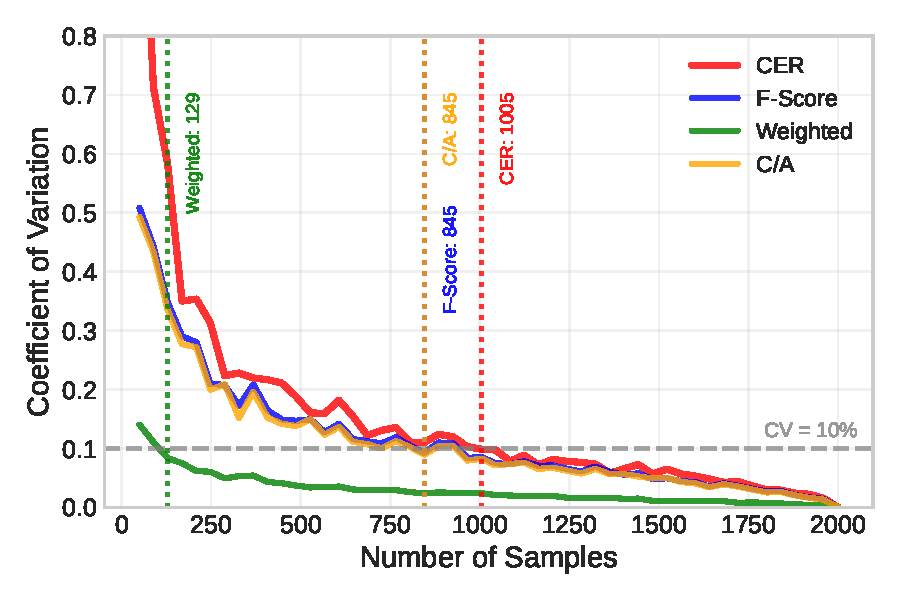
\includegraphics[width=\textwidth]{Figures/cv_comparison.pdf}
        \vspace{0.8em}
        \caption{Coefficient of variation of RI when evaluating on subsets of the full dataset. \cm{Add significance test}}
        \label{fig:refusal_index_cv_subset}
    \end{minipage}
    \hfill
    \begin{minipage}[t]{0.48\textwidth}
        \centering
        \vspace{-18.8em}
        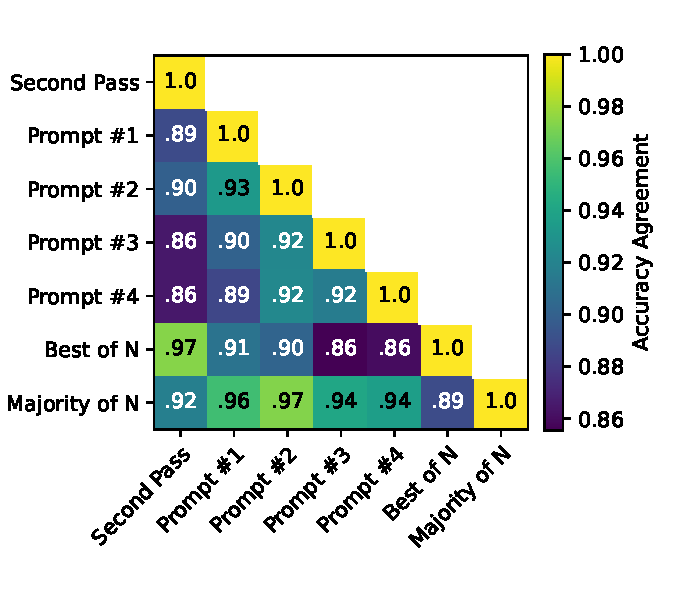
\includegraphics[width=\textwidth]{Figures/prompt_acc_agreement.pdf}
        \caption{Accuracy agreement between different prompt strategies.}
        \label{fig:prompt_acc_agreement}
    \end{minipage}
\end{figure}

We next examine how variations in prompt design affect the RI evaluation. Our experimental setup uses four distinct first-pass prompts, each with different few-shot examples and instructions, to induce varying refusal rates. For the second pass, a single, simpler prompt is used to compel the model to answer all previously refused questions. Although these prompts are designed to produce different refusal rates, it is crucial to verify that they do not introduce confounding effects on model accuracy, which would in turn impact the RI calculation.

To assess this, we measure the accuracy agreement between pairs of prompt strategies. Agreement is calculated as the proportion of questions for which both prompts yielded the same correctness label, considering only the questions answered by both. As shown in Figure~\ref{fig:prompt_acc_agreement}, the accuracy agreement between different first-pass prompts is consistently high (over 90\%). This indicates that the choice of prompt strategy does not significantly alter the model's underlying accuracy on the questions it chooses to answer. Furthermore, the high agreement involving the forced-answer (second-pass) prompt validates its use for effectively estimating the model's baseline accuracy ($\mu$).